\section{PIR框架设计}
\label{sec:pir-framework}

本节将详细讨论基于纠删码分区的PIR协议框架细节,包括框架的设计思想和具体工作流程。

\subsection{框架设计}
整体框架工作流程如图\ref{fig:pir-framework-lane}所示。

\begin{figure}
    \centering
    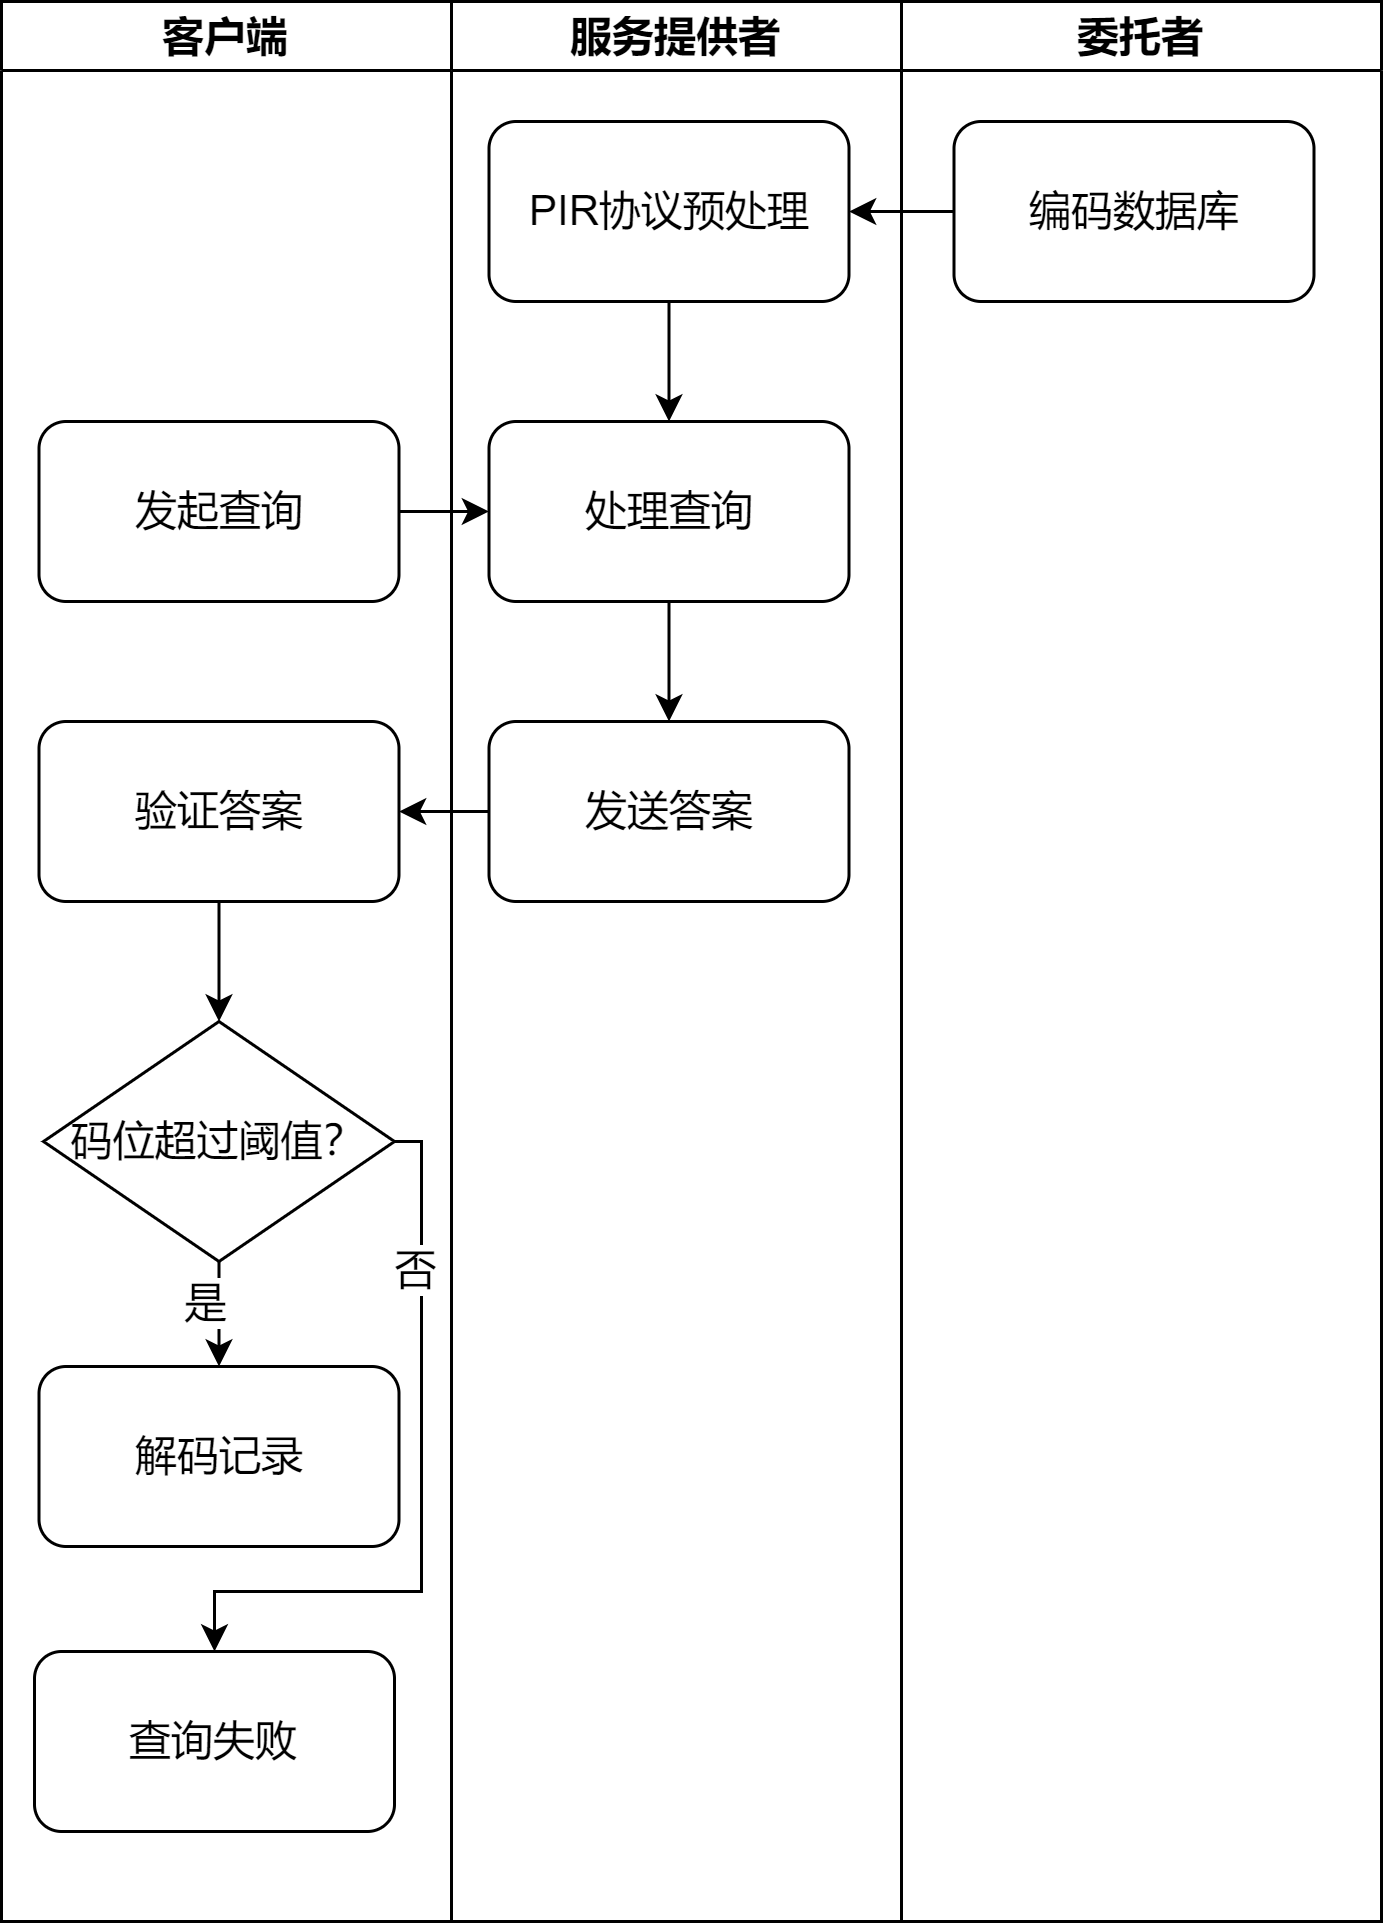
\includegraphics[width=0.8\textwidth]{figure/查询框架泳道图.png}
    \caption{PIR框架泳道图}
    \label{fig:pir-framework-lane}
\end{figure}

数据库经编码后分发至多个服务器,每个服务器独立处理PIR请求,最终客户端将结果解码为原始记录。在此过程中,编码和解码需要遵循相应的对应关系,使用相同的编解码方式,对于PIR协议的选择比较灵活,出于前述原因,我们要求PIR协议能够支持验证,但不对PIR的具体流程和复杂性做硬性规定。本文默认采用第\ref{sec:construction}节中提出的协议作为框架内的PIR协议。

\subsection{框架具体流程}
在编码阶段,有两种分组方式可以使用:
\begin{itemize}
    \item 保持单条记录大小不变,以多条记录为单位进行编码,将原本大小为$\dbsize\times\recordsize$的数据库编码为$\servercount$个大小为$\frac{\dbsize}{\servercount-\threshold}\times\recordsize$的子数据库。
    \item 保持记录条数不变,以单条记录中的比特为单位进行编码,将原本大小为$\dbsize\times\recordsize$的数据编码为$\servercount$个大小为$\dbsize\times\frac{\dbsize}{\servercount-\threshold}$的子数据库。
\end{itemize}

两种方式各有优劣。从复杂度的角度来看,单次查询的计算和通信与记录大小成正比,与记录条数的平方根成正比,保持记录条数不变更有优势。从通信量构成的角度来看,保持单条记录大小不变降低了客户端向服务器的请求大小,而保持记录条数不变降低了客户端从服务器收到的回复大小。实践中,考虑到下述原因,本文采用了保持单条记录大小不变的方式:
\begin{enumerate}
    \item 保持单条记录大小不变更具有可拓展性。随着数据库增大,可以使用更多的服务器进行扩容。如果保持记录条数不变,则服务器的数量上限受到单条记录的大小限制,尤其在单条记录较小时无法有效分组。
    \item 亚线性PIR协议与较小的记录兼容性不佳。与线性PIR协议不同,亚线性PIR访问的地址不连续,很难采用向量化、SIMD指令等方式加速运算。因此,即便单条记录很小,协议也必须单独计算。虽然记录变小后也能降低单条记录的处理时间,但访存、计算、通信等时间存在下限。换言之,当记录被分割得足够小时,进一步分割记录就无法加速PIR协议运行了。
\end{enumerate}

框架具体执行流程如图\ref{fig:framework-protocol}所示:
\begin{figure*}
    \begin{mdframed}
        \paragraph{符号约定:} 协议包含一个客户端 $\client$ 与共 $\servercount$ 台服务器 $\server_0, \server_1, \dots, \server_{\servercount-1}$,底层PIR协议 $\Pi = (Setup, Query, Answer, Reconstruct)$。如果使用的PIR协议是一离线-在线PIR协议,其中 $Hint$ 被包括于 $Setup$ 中,$Refresh$ 被包括于 $Reconstruct$ 中。协议运行于包含 $\dbsize$ 条记录的数据库 $\db$ 上。为保证可靠性,我们期望能够容忍最多 $\threshold$ 台服务器掉线或出错。不妨设 $\servercount - \threshold$ 整除 $\dbsize$。如此条件不能满足,可以向数据库填充空白记录。将 $(\servercount - \threshold, \servercount, \threshold)$ 纠删码方案记为 $\Pi_c = (Encode, Decode)$。

        \begin{itemize}
            \item \textbf{预处理阶段:} 服务器共同将数据库$\db$按$\servercount-\threshold$条记录大小分组,每组使用$Encode$算法编码为$\servercount$个元素,共$\frac{\dbsize}{\servercount-\threshold}$组。每组的第$i$个元素存储在第$i$台服务器上。完成后,每台服务器应持有大小为$\frac{\dbsize}{\servercount-\threshold}$的数据库。每台服务器使用自己的数据库运行$Setup$算法(包括可能存在的$Hint$)。
            \item \textbf{查询阶段:} 设客户端查询的记录索引为$\dbidx$。客户端与每台服务器分别运行$Query(\lfloor\frac{\dbidx}{\servercount-\threshold}\rfloor)$,服务器调用$Answer$给出答案,客户端调用$Reconstruct$获得共$\servercount$个答案$x_0, x_1, \dots, x_{\servercount-1}$。由于验证的原因,其中部分答案可能是$\bot$。
            \item \textbf{解码阶段:} 客户端调用$Decode$将共$\servercount$个答案解码为$\servercount-\threshold$条记录,并找到对应$\dbidx$的记录。如果$\bot$答案数超过$\threshold$,客户端输出$\bot$。
        \end{itemize}
    \end{mdframed}
    \caption{基于编码的PIR协议框架具体执行流程}
    \label{fig:framework-protocol}
\end{figure*}

\paragraph{框架的进一步优化}
在协议中,如果服务器不产生任何私有状态,客户端可以与所有服务器使用相同的随机数进行交互。具体到本文的PIR协议,这意味着客户端可以使用相同的PRF密钥在$Hint$算法中与每台服务器交互,获得完全相同的Hint集合,仅在校验值上有所差异。在线阶段,调用$Query(\lfloor\frac{\dbidx}{\servercount-\threshold}\rfloor)$生成的查询可以在所有服务器上通用。这一优化的正确性和安全性可以直接从\ref{sec:framework-assumption}节中的假设得到。

这种优化带来了许多好处:
\begin{enumerate}
    \item 由于$Query$算法的结果可以通用,客户端无需重复运行$Query$算法,只需多次进行$Reconstruct$算法。其在线计算量绝大部分与服务器总数无关,仅与每台服务器持有的数据库大小有关。
    \item 所有服务器使用相同的PRF密钥,客户端可以减少集合PRF密钥的存储量。
    \item 客户端的请求可以被转发。如果一台服务器负责转发请求和回复,分布式服务器可以对客户端透明。客户端无需知道所有服务器的地址以发出请求,只需将请求发送给中继服务器以处理。
\end{enumerate}

此外,如果将单服务器PIR协议作为PIR框架的基础,客户端在离线阶段也可以使用未编码的数据库,自行运行编码阶段和离线阶段,以避免与多台服务器运行离线阶段。由于此阶段,服务器的瓶颈在于网络带宽而非硬盘读写,服务器无需将整个数据库加载到内存中,对服务器的内存并无硬性要求。然而,这要求至少有一台服务器完整存储了整个数据库,并非在所有情况下都适用。

\subsection{支持数据库更新}

处理数据库的增删改可以简单概括为对子数据库的增删改,其细节我们已经在第\ref{sec:handling-updates}节中讨论过。仅剩的问题是如何处理服务器的增减。在此,我们将分两类情况进行讨论:
\begin{itemize}
    \item \textbf{修改服务器数量,但不改变数据分组方式:}在采用Reed-Solomon编码时,这种修改是比较简单的。新增的服务器需要与现有的服务器协商得到自己的子数据库,但其他服务器的数据不需要改动。在删除服务器时,不需要进行任何额外的操作。
    \item \textbf{修改数据分组方式:}这需要所有服务器共同重新执行预处理阶段。
\end{itemize}

